\chapter{環境}	
\thispagestyle{plain}   % chapterの直後に必ず指定

本章では,本研究のゲーム環境であるMinecraftやテスト環境のFUN Minecraft Serverについて述べる.

\section{Minecraftとは}\label{sec:minecraft}
Minecraft\cite{bib:Minecraft}とは,創造性やサバイバル生活に焦点を当てた,サンドボックス型のゲームである.Minecraftの世界は図\ref{fig:mc_world}のように,3D空間で水平方向にほぼ無限に広がっており,木,石,土,水など様々な種類の一定の大きさの立方体ブロックで構成され,その世界にはドット絵調の動植物が存在する.プレイヤーは主に以下の二つのモードでゲームを楽しむことができる.\\

\textbf{サバイバルモード} 冒険と生活を主体としたモードである.体力や空腹度の概念が存在するため,プレイヤーは死を免れるために狩猟,採集,農業,牧畜などで食料を収集し,ブロックの収集や集めたアイテムの加工 (クラフト)を駆使して敵から逃れるための安全な住居を作らなければならない.\\

\textbf{クリエイティブモード} ブロックの組み立てに重きをおいた,創造性や実験を主体としたモードである.サバイバルモードと比較して,体力や空腹度の概念がなく,組み立てがしやすいように自由に飛行することが可能である.また,すべてのブロックを無限に配置でき,瞬時に破壊することが可能である.したがって,サバイバルモードでは制作困難な巨大建築や,複雑な回路の作成を楽しむことが可能となっている.\\
\begin{figure}[H]
    \centering
    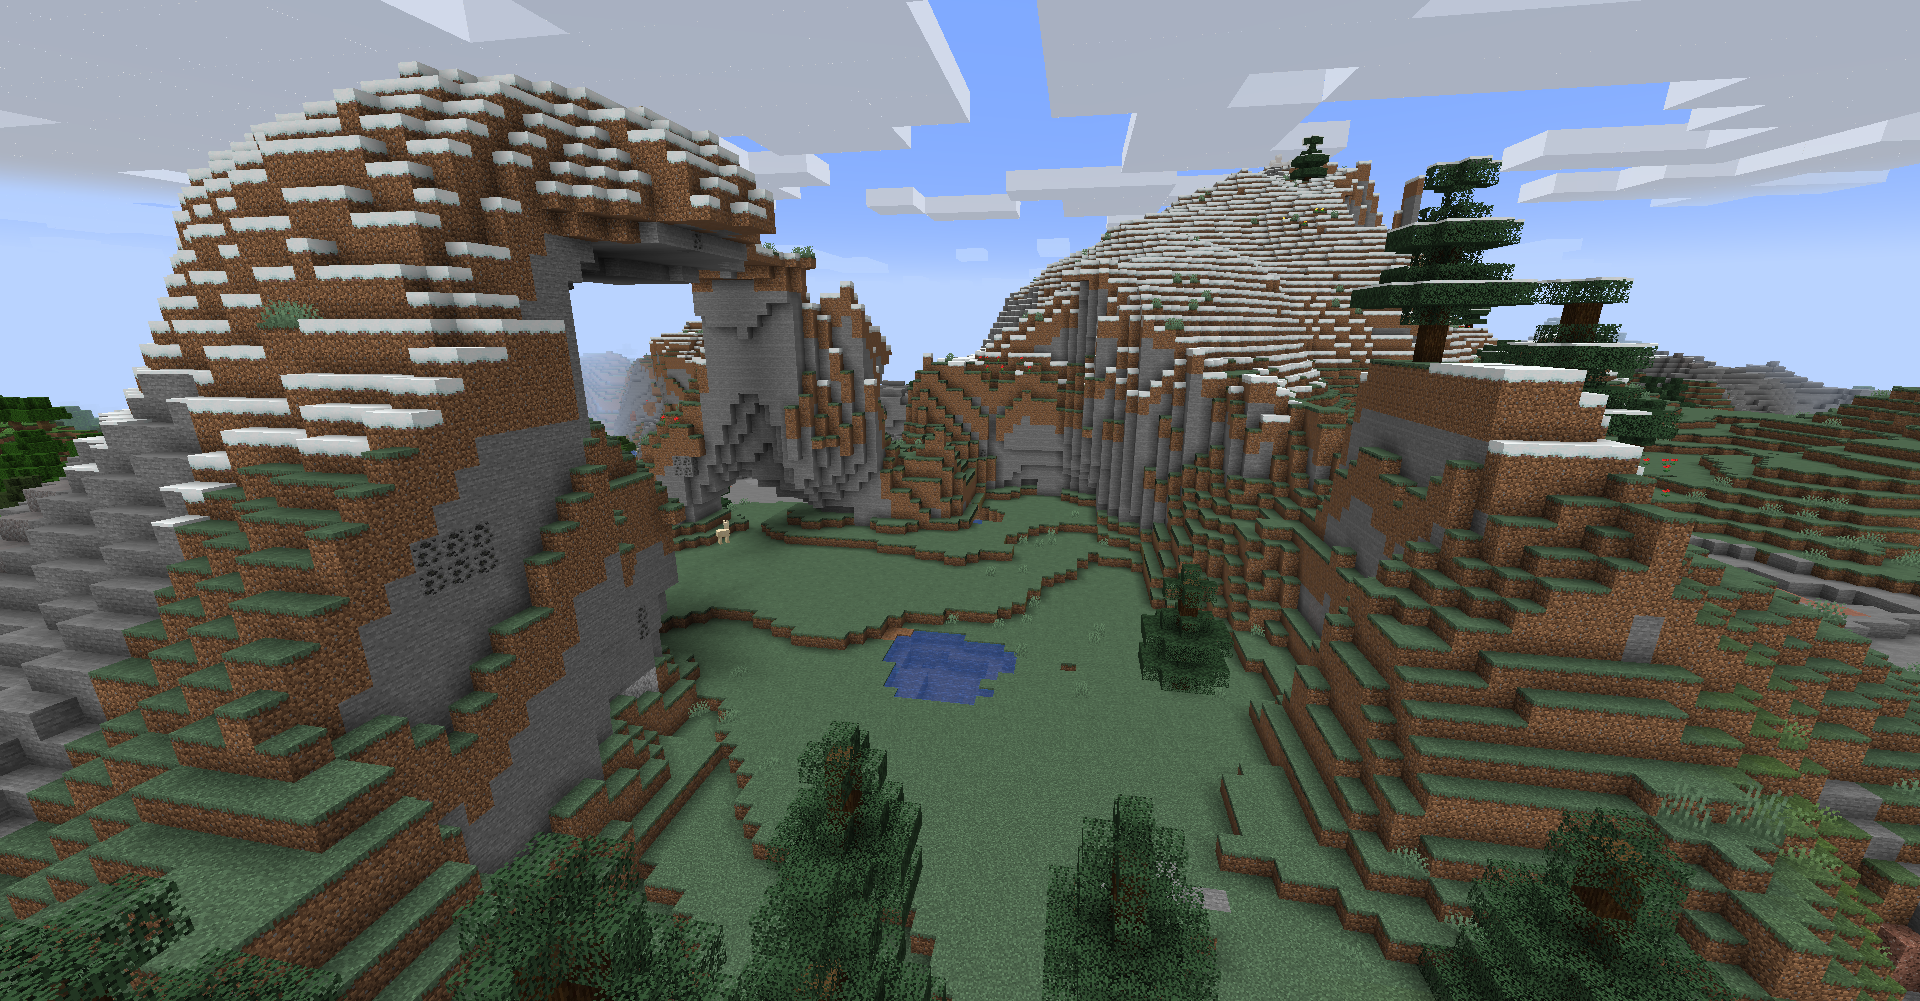
\includegraphics[width=0.7\textwidth]{fig/minecraft_world.png}
    \caption{Minecraftの世界}
    \label{fig:mc_world}
\end{figure}

\section{Minecraftの特徴}\label{sec:minecraft_feature}
Minecraftには,以下のような学術的に有利な特徴がある.\\

\textbf{認知度} Minecraftは2011年にPCで正式版がリリースして以来,iOSやAndroidなどのスマートフォン機種や,Xbox One,Nintendo Switchなどの家庭用ゲーム機,その他様々なプラットフォームに移植された.
また,2023年10月にはMinecraftの累計売り上げ本数が3億本を突破したことが公式ライブで発表され,世界で最も売れたインディーゲームとなった\cite{bib:minecraft_news}.
このように対応するプラットフォームが多く認知度が高いことから,ゲームのルールや特徴を知っている人が多いと予想できるため,評価実験やアンケートなどの客観的尺度が必要になった場合には遂行しやすくなることが考えられる.\\
%TODO: いつだったかの発表の好きな実況ゲームランキング入れる

\textbf{ゲーム環境} Minecraftは特定の目標がなく,オープンワールドであるため,AIの行動の可能性を広げることが可能である.
また,場合によってはブロックの設置により,逆に行動を制限させ,柔軟にAIの学習環境を設定することが可能である.\\

\textbf{拡張性} Minecraftは拡張機能 (MOD) やツールの種類が多く,Minecraft最大手のMOD公開サイトとなっているCurseForge\cite{bib:curseforge}では,2024年1月現在で約153,204のMODプロジェクトが公開されている.
多くのMODが開発されている理由として,Minecraft EULA\cite{bib:eula}ではMinecraftのMOD (プログラムの修正,ツール,プラグイン含む)の追加を許可しており,開発のためのコミュニティも活発であることが挙げられる.
したがって,拡張性が高いため研究に合わせてゲーム性を保ったまま自由にMinecraftをカスタムすることが可能である.\\

\textbf{教育的価値} サバイバルや建築を楽しむことが可能であるゲーム性から,問題解決力や創造性を養うことが可能である.
その教育性からMinecraft公式は,Minecraft Education (教育版マインクラフト)\cite{bib:minecraft_edu}をリリースしている. \\

\section{FUN Minecraft Serverについて}
FUN Minecraft Server\cite{bib:fun_minecraft_server}は,公立はこだて未来大学の協力と支援のもとで成り立っている公認のサーバーである.
複数の研究室と多くの有志メンバーから「Minecraftを用いた数多くの研究に繋がる可能性」への共感を得て,実現が可能となった.
FUN Minecraft Serverは,MinecraftのJava版のアカウントを取得しており,公立はこだて未来大学に所属している人であれば参加することが可能である.
FUN Minecraft Serverプロジェクトの目的は,FUN Minecraft Serverのオンライン環境を通して,公立はこだて未来大学に所属する学生や教員が研究のアイデアの着想を得ることである.
海外の大学では,同様の目的でMinecraftの大学公式サーバーを運用する事例が複数あり,効果的な成果があったと報告されている\cite{bib:cambridge_minecraft_server, bib:texas_minecraft_server}.
国内の大学におけるMinecraftの公式サーバー運用に関する事例は,FUN Minecraft Serverと同時期に設立されたプロジェクトが確認された\cite{bib:tducraft}.しかし,そのような事例は依然として限られており,その実施は比較的稀であると言える.
したがって,FUN Minecraft Serverが国内の大学の公式サーバのモデルケースになる可能性が期待される.

実際にFUN Minecraft Serverは様々な研究の環境として利用されている.
本研究で作成した{\mason}もFUN Minecraft Serverを動作テストやアンケートを行うための環境として用いている.
過去には,Minecraftで作成したビデオを使用して,小学生向けの教材を作成した研究が存在していた\cite{bib:fun_minecraft_server_research}.
また,現行の研究では,BEVI-J評価ツールを使用して,FUN Minecraft Serverに参加した学生の人物像についての研究\cite{bib:fun_minecraft_server_research}や,運営側でサーバーにPlan,CoreProtect,DiscordSRVなどのプラグインを導入し,コミュニティをモニタリング・管理し,ゲームプレイデータを収集・分析する研究などが行われている\cite{bib:fun_minecraft_server_research,bib:fun_minecraft_server_research2}.